\section{Vacuum}
\subsection{Requirements and Tasks}

The main task of the vacuum team is to design a vacuum chamber that can be used for a small table top stellarator.
For this the maximum size of the chamber was given, so it can fit through a standard door of (90 x 200)~cm.
Thus this are the maximum dimensions of the individual parts of the chamber.

The necessary requirements for the chamber are:
(a) The chamber should be large enough to fit the coils for the stellarator as well as all other devices to generate and measure the plasma,
(b) needs to be able to withstand pressures $<\SI{e-8}{\milli\bar}$, when evacuated,
(c) should be able to encounter different types of noble gases to create the plasma,
(d) should be able to withstand the radiation of the plasma as well the microwave radiation of the heating. \\

In order to achieve these requirements, the focus is on the design of the vacuum chamber, the vacuum system, and the radiation protection.
This is described in more detail in the full \href{https://www.overleaf.com/3861427278qpnrdmbhknty#518852}{\emph{Vacuum Team Report}}.
This report also includes the design process, description of the most important ports and feedthrough, the vacuum system, and the radiation protection.
Here only a brief overview of the most important1 aspects is given.

\subsection{Outcome}

\subsubsection{Vacuum chamber}

The design of the vacuum chamber, which was finalized, is shown in \autoref{fig:Kammer_all}.
It has a dome shaped lid as well as a dome shaped base.
This allowed to increase the size of the chamber as the base and the lid are both removable and can be placed together inside a laboratory.
The given specifications of the size were given, that the chamber need to fit through a standard door, with the size of (90 x 200)~cm.
Also other configuration were considered, for example with a flat base and a flat lid, but the dome shaped design was chosen as it was the most rigid one.
The rigidity is needed to prevent the chamber from bending when evacuated to a pressure of~$<\SI{e-8}{\milli\bar}$.

For the sake of simplicity, all flange connections were chosen to have the same size.
Only the connections for the Pirani-Bayard-Alpert pressure measurement and the quadrupole spectrometer were chosen differently, as little was previously known of specific flange sizes.
The universal fange connections chosen for the versatile connection is the same flange used as for the TMP (DN 320 ISO-F).
This flange size was chosen because if a second TMP is needed, it can be easily added to the chamber using a knee.
Also the relative large size of the flange allows to connect other flanges to it using adapters.

Apart from the ports already known for the chamber, additional ports with standard flanges are added.
This makes is easier for the future use of the chamber, as retrofitting extra ports is not necessary.
Also adding ports from the beginning makes it cheaper, as not much work is needed to add them later on.

To support the wight of the chamber, foots are added to the side of the vessel.
This will allow to place the entire chamber on a steel scaffold.
Thus, these mounts need to be able to support the entire weight of the chamber as well as the weight of the external mounted devices.
%\todo{add foot mounts of the chamber (description)}

\begin{figure}[H]
    \centering
    \begin{subfigure}[b]{0.4\textwidth}
        \centering
        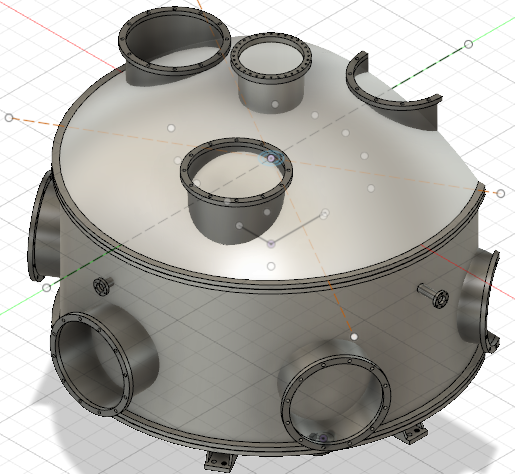
\includegraphics[width=1\textwidth]{Images/06_Vacuum/Vakuumkammer_final.PNG}
        \subcaption{Final version of the vacuum chamber.}
        \label{fig:Kammer}
    \end{subfigure}
    \hfill
    \begin{subfigure}[b]{0.4\textwidth}
        \centering
        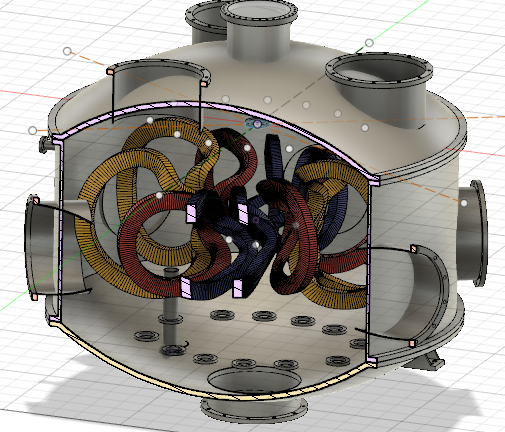
\includegraphics[width=1\textwidth]{Images/06_Vacuum/Vakuumkammer_final_Schnitt.PNG}
        \subcaption{Sectional analysis of the chamber: The flanges for the coil connections facing inwards are visible on the inside. }
        \label{fig:Kammer_Schnitt}
    \end{subfigure}
    \caption{Views of the completed vacuum chamber at the status of the 10.07.2024.}
    \label{fig:Kammer_all}
\end{figure}


\subsubsection{Vacuum design}


For the Vacuum system a turbo-molecular pump is chosen, due its oil-free operation and pumping speed.
It is backed up by a sufficiently sized backing pump which also provides the rough vacuum before the TMP takes over.
To reduce outgassing metal surfaces in the inside are polished and wires are heat and electrically isolated by using e.g. Kapton$\textsuperscript{\textregistered}$.
Pressure is measured using a pressure gauge that includes a Pirani device for lower vacuum levels and a Bayard-Alpert device for higher vacuum ranges.
For a residual gas analysis one port is reserved for hosting a quadrupole mass spectrometer.


\subsubsection{Radiation protection}

The vacuum vessel is designed with a thickness of $\SI{10}{\milli\meter}$, which provides adequate protection against X-ray and microwave radiation. The chosen material is austenitic stainless steel 316L. This material was selected due to its non-magnetic nature and its advantageous properties, including high strength, good availability, and overall versatility, making it an ideal choice for our application.

The window was designed with a circular shape having a radius $\SI{100}{\milli\meter}$ made of quartz glass. The ideal thickness for the window is $\SI{10}{\milli\meter}$.


\subsection{Outlook}

It is important to perform a detailed structural analysis to ensure the chamber can withstand external atmospheric pressure and any mechanical stresses without significant deformation or failure.
Moving forward, the design of the vacuum chamber may need to be adjusted based on the specific requirements of the other teams involved in the design process.
The exact number and types of ports, as well as other components such as windows, gas inlets, feedthroughs, and coaxials, have not been finalized yet.
Therefore, additional work will be needed to finalize these details and to ensure that the vacuum chamber design meets all necessary requirements.
It is also necessary to ensure that the design meets relevant safety standards and regulations for vacuum systems and radiation protection.
Safety features such as emergency shutdown systems and radiation monitoring should be included.
For this reason, integration of various sensors and instrumentation for monitoring temperature, radiation levels and other critical parameters should be considered.
Moreover, it is essential to develop safety protocols for handling and maintenance, ensuring personnel are aware of and protected from potential radiation exposure.
At this stage, the cost of the vacuum chamber itself remains unknown and cannot be estimated.
The manufacturer does not provide list prices for such custom-made items and would only provide a cost estimate upon specific order inquiry.
It is anticipated that the vacuum chamber itself would represent one of the largest expenses for the entire project, primarily due to the necessity of custom manufacturing.

\subsection{Learnings}

Designing the vacuum chamber for a small stellarator has provided significant insights into project management.
This includes conducting independent research and efficiently integrating findings into our design decisions.
Recognizing the importance of considering diverse perspectives and requirements from other teams involved was both challenging and instructive.
Collaborating closely with other teams emphasized the importance of sharing skills and expertise, resulting in a more cohesive project outcome.
